\documentclass[hyperref=unicode]{beamer}

% preklad provadet pdfcsLaTexem

\usepackage[absolute,overlay]{textpos}
\usepackage{graphicx}
\usepackage{adjustbox}
\usepackage{mhchem}
\usepackage{ucs}
\usepackage[utf8]{inputenc}
\PrerenderUnicode{ěščřžýáíéĚŠČŘŽÝÁÍÉďťňĎŤŇůúÚóÓ}

\adjustboxset*{center}

% balicek s cestinou
\usepackage[czech]{babel}
%\usepackage[english]{babel}
% hyperodkazy (zrejme neni nutne)
%\usepackage{hyperref}
% fonty pro matematicke vzorce
%\usepackage{amsfonts}


% mod pro prezentaci, pouzije se tema (rozvrzeni) Darmstadt (nahradit podle libosti za jine)
\mode<presentation>{\usetheme{default}}
% lze volat i \mode<presentation>{ \usetheme{Darmstadt} \usecolortheme{dove}}

% prehled vychozich dostupnych temat(rozvrzeni) (nutne zadat vcetne velikosti pisem):
% AnnArbor, Antibes, Bergen, Berkeley, Berlin, Boadilla, boxes, CambridgeUS, Copenhagen, Darmstadt, default, Dresden, Frankfurt, Goettingen, Hannover, Ilmenau, JuanLesPins, Luebeck, Madrid, Malmoe, Marburg, Montpellier, PaloAlto, Pittsburgh, Rochester, Singapore, Szeged, Warsaw

% prehled vychozich dostupnych barevnych temat(nutne zadat vcetne velikosti pisem):
% albatross, beaver, beetle, crane, default, dolphin, dove, fly, lily, orchid, rose, seagull, seahorse, sidebartab, structure, whale, wolverine



% definice barvy pozadi vsech snimku
% jednotlive barevne slozky:
% R= 0 az 255, G= 0 az 255, B= 0 az 255
% \DefineNamedColor{named}{pozadi}{RGB}{R,G,B}
% prednastavena svetle modra barva
\DefineNamedColor{named}{pozadi}{RGB}{200,200,200}

% nastavi barvu pozadi ve vsech snimcich na barvu definovanou v predchozim kroku
\setbeamercolor{background canvas}{bg=pozadi} 

\RequirePackage{czech}
% pouzije vlastni sablonu vzhledu (sazba titulni stranky)
%\usepackage{VUTobhajoba}

\setbeamertemplate{footline}[frame number]


\begin{document}
\title[Crisis] % (optional, only for long titles)
{Praktické využití IR spektroskopie}

\author % (optional, for multiple authors)
{Zdeněk Moravec}
\date[KPT 2004] % (optional)
{20. listopadu 2014}

\frame{\titlepage}

% snimek s cili (zadanim) prace


\frame{
	\frametitle{Osnova}
	\vfill
	\begin{itemize}
	\item Základní principy IR spektroskopie
	\item Měřící techniky
	\begin{itemize}
		\item FT-IR transmisní měření
		\item ATR, DRIFT, PAS
		\item TG/IR, GC/IR
	\end{itemize}
	\item Zpracování spekter
	\begin{itemize}
		\item Analýza spekter
		\item Spektrální databáze
	\end{itemize}
	\item Aplikace
	\begin{itemize}
		\item Chemie
		\item Restaurování uměleckých předmětů
		\item Biologie
	\end{itemize}
	\item Informace o přístrojovém vybavení UCH
	\end{itemize}
	\vfill
}

\frame{
	\frametitle{Molekulová spektroskopie}
	\vfill
	\begin{tabular}{|p{2.2cm}|p{3cm}|p{2cm}|p{2cm}|}
	\hline
	& UV-VIS & IR & MW \\
	& 50-800 nm & 1-100 $\mu$m & 1-10 mm \\
	\hline
	Elektronická
	\newline spektroskopie & Absorpční UV-VIS 
	\newline Luminiscenční spektroskopie & & \\
	\hline
	Vibrační 
	\newline spektroskopie & Ramanova spektroskopie & Infračervená spektroskopie & \\
	\hline
	Rotační 
	\newline spektroskopie & Ramanova spektroskopie & & Mikrovlnná spektroskopie \\
	\hline
	\end{tabular}
	\vfill
}


\frame{
	\frametitle{Základní principy IR spektroskopie}
	\vfill
	\adjincludegraphics[width=250pt,valign=t]{img/em-spectrum.png}
	\vfill
}

\frame{
	\frametitle{Základní principy IR spektroskopie}
	\vfill
	\adjincludegraphics[width=250pt,valign=t]{img/el-prechody.png}
	\vfill
}

\frame{
	\frametitle{Vibrace chemických vazeb}
	\vfill
	\begin{itemize}
	\item Během vibrace vazby dochází k přechodu systému na jinou energetickou hladinu.
	\item Přechod mezi základní a 1. excitovanou hladinou se nazývá \em základní (fundamentální) vibrace \em.
	\item Pokud dochází k přechodům na vyšší hladinu, jedná se o tzv. \em vyšší harmonické přechody (overtony) \em. Jejich frekvence jsou \em přibližně \em násobkem fundamentální frekvence (energetické hladiny se postupně zhušťují).
	\item Pokud dojde k současné změně dvou vibračních stav molekuly jedná se o \em kombinační přechody \em.

	\end{itemize}
	\vfill
}

\frame{
	\frametitle{Valenční a deformační vibrace}
	\vfill
	\begin{itemize}
	\item Valenční vibrace – dochází ke změně mezijaderné vzdálenosti.
	\item Deformační vibrace – dochází ke změně vazebného úhlu.
	\end{itemize}
	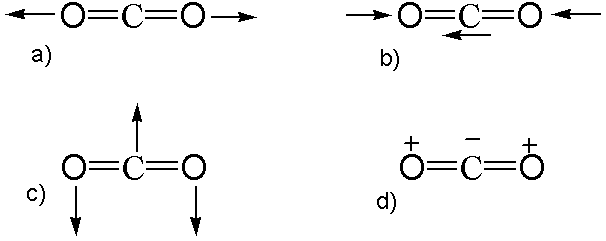
\includegraphics[scale=0.4]{img/CO2-vibration.png}
	\vfill
}

\frame{
	\frametitle{Absorpce infračerveného záření}
	\vfill
	\begin{itemize}
	\item Aby mohla molekula absorbovat infračervené záření musí během vibrace docházet ke změně dipólového momentu.
	\item Při absorpci dochází ke změně amplitudy vibrace, frekvence zůstává nezměněna.
	\item Intenzita absorpčních pásu je úměrná druhé mocnině změny dipólového momentu.
	\item Absorpcí infračerveného záření molekulami vznikají pásová spektra.
	\end{itemize}
	\vfill
}

\frame{
	\frametitle{Infračervená spektroskopie}
	\vfill
	\begin{itemize}
	\item  NIR (0,7 -- 2,5 $\mu$m; 14 000 - 4 000 cm$^{-1}$) - infračervená spektroskopie v blízké oblasti
	\item  MIR (2,5 -- 25 $\mu$m; 4 000 - 400 cm$^{-1}$) - infračervená spektroskopie ve střední oblasti
	\item  FIR (25 -- 1000 $\mu$m; 400 - 10 cm$^{-1}$) - infračervená spektroskopie ve vzdálené oblasti
	\end{itemize}
	\vfill
}

\frame{
	\frametitle{Absorpční spektrum}
	\vfill
	\adjincludegraphics[width=300pt,valign=l]{img/spectrum.png}
	\begin{textblock*}{1cm}[1,1](55mm,65mm)
	
\includegraphics[width=80pt]{img/spectrum-struct.png}
	\end{textblock*}
	\begin{itemize}
	\item Absorpční spektrum indiga
	\end{itemize}
	\vfill
}

\frame{
	\frametitle{Měřící techniky}
	\vfill
	\begin{itemize}
	\item  FT-IR - transmise, ATR
	\item  DRIFT, IRRAS
	\item TG-IR, GC-IR
	\end{itemize}
	\vfill
}

\frame{
	\frametitle{FT-IR}
	\vfill
	\begin{itemize}
	\item  Nejběžnější měřící technika
	\item Podle úpravy vzorku rozlišujeme měření v transmisním módu a ATR
	\item Spektrometr neobsahuje monochromátor, ale interferometr
	\item Celé spektrum se snímá najednou, získáme interferogram, který je nutné zpracovat pomocí Fourierovy transformace
	\end{itemize}
	\vfill
}

\frame{
	\frametitle{FT-IR}
	\vfill
	\adjincludegraphics[width=11cm,valign=l]{img/ftir.png}
	\vfill
}

\frame{
	\frametitle{Transmisní měření}
	\vfill
	\begin{itemize}
	\item  Lze měřit pevné látky, kapaliny i plyny
	\item Pevné látky měříme ve formě KBr tablet (1-3 hm. \% v KBr) nebo jako suspenze v Nujolu
	\item Kapaliny měříme jako tenký film mezi okny z vhodného materiálu (KBr, KRS, NaCl, ...)
	\end{itemize}
	\adjincludegraphics[width=300pt,valign=l]{img/kbr-pellets.png}
	\vfill
}

\frame{
	\frametitle{Transmisní měření - Nujol}
	\vfill
	\begin{itemize}
	\item Nujol - směs alkanů s dlouhý řetězcem.
	\end{itemize}
	\adjincludegraphics[width=300pt,valign=l]{img/nujol.png}
	\vfill
}

\frame{
	\frametitle{Transmisní měření}
	\vfill
	\begin{itemize}
	\item Plyny se měří v plynových kyvetách, ty jsou konstruované tak, aby dráha paprsku byla co nejdelší
	\item Protože v plynném skupenství existují pouze slabé interakce mezi částicemi lze naměřit čistě rotační, rotačně-vibrační i elektronově-rotačně-vibrační spektra
	\end{itemize}
	\adjincludegraphics[width=90mm,valign=l]{img/water.png}
	\vfill
}

\frame{
	\frametitle{ATR}
	\vfill
	\begin{itemize}
	\item ATR - Attenuated Total Reflection
	\item Krystaly jsou z diamantu, ZnSe, Ge, KRS-5 (směs TlBr a TlI) nebo křemíku
	\item Vzorek se přitlačí vysokým tlakem k měřícímu krystalu
	\item Paprsek se pohybuje po povrchu vzorku (0,5 - 5 $\mu$m)
	\end{itemize}
	\vfill
	\adjincludegraphics[width=180pt,valign=b]{img/atr.png}
}

\frame{
	\frametitle{IRRAS}
	\vfill
	\begin{itemize}
	\item IRRAS - IR Reflection Absorption Spectroscopy
	\item Metoda vhodná pro tenké vrstvy nanesené na kovových materiálech nebo nasorbované látky na materiálech
	\item Pro zvýšení citlivosti se využívá polarizovaného záření
	\end{itemize}
	\adjincludegraphics[width=200pt,valign=l]{img/irras.png}
	\vfill
}

\frame{
	\frametitle{DRIFTS}
	\vfill
	\begin{itemize}
	\item DRIFTS - Diffuse Reflectance Infrared Fourier Transform Spectroscopy
	\item Tato technika je vhodná pro měření malých částic nebo hrubých povrchů
	\item Využívá rozptylu IR záření
	\item Rozptýlené záření je pomocí kulového zrcadla odráženo na detektor
	\item Práškové vzorky se měří v kelímcích, pevné vzorky se obrousí abrasivem (SiC) a měří se částice zachycené na abrasivu
	\end{itemize}
	\adjincludegraphics[width=52mm,valign=l]{img/drifts.png}
	\vfill
}


\frame{
	\frametitle{Coupling TGA/IR}
	\vfill
	\begin{itemize}
	\item TGA - termogravimetrická analýza
	\item Plyny vznikající během degradace vzorku vedeme do měřící cely a pomocí IR spektroskopie stanovíme jejich složení
	\item Během transportu plynů z pece do měřící cely dochází k velkému zředění plynu, proto je nutné používat citlivější detektory (MCT)
	\end{itemize}
	\adjincludegraphics[width=10cm,valign=l]{img/tg-irFoto.jpg}
	\vfill
}

\frame{
	\frametitle{Coupling TGA/IR}
	\vfill
	\adjincludegraphics[width=11cm,valign=l]{img/tg-ir.png}
	\vfill
}

\frame{
	\frametitle{Coupling GC/IR}
	\vfill
	\begin{itemize}
	\item GC - plynová chromatografie
	\item Méně citlivé než GC/MS, ale umožňuje analýzu stereoizomerů.
	\item Interferogramy je nutné snímat v krátkých časových intervalech
	\end{itemize}
	\adjincludegraphics[width=10cm,valign=l]{img/gc-ir.jpg}
	\vfill
}

\frame{
	\frametitle{Analýza spekter}
	\vfill
	\begin{itemize}
	\item Oblast otisku prstu – 500 – 1500 $cm^{-1}$
	\begin{itemize}
		\item valenční vibrace většiny anorganických molekul
		\item deformační vibrace organických molekul – $\delta$ HCH, $\delta$ CCH, $\delta$ COH
		\item některé valenční vibrace organických molekul $\nu$ C-C, $\nu$ C-O
	\end{itemize}
	\item Charakteristické vibrace – poloha spektrálních pásů funkčních skupin je relativně málo závislá na zbytku molekuly, proto je možné jejich vlnočty tabelovat
	\end{itemize}
	\vfill
}

\frame{
	\frametitle{Tabulky vlnočtů}
	\vfill
	\adjincludegraphics[width=115mm,valign=l]{img/tab.png}
	\vfill
}

\frame{
	\frametitle{Analýza spekter}
	\vfill
	\begin{itemize}
	\item Izotopicky obohacené molekuly
	\begin{itemize}	
		\item Izotopická substituce usnadňuje interpretaci vibračních spekter
		\item Nedochází ke změně geometrie molekuly, ale změní se hmotnost atomů a tím i poloha absorpčních pásů
	\end{itemize}
	\item Analýza vodíkových vazeb
	\begin{itemize}	
		\item \ce{R\bond{-}O\bond{-}H\bond{...}O} $\nu$(OH) = 3500-2500 cm$^{-1}$
		\item \ce{R\bond{-}O\bond{-}H} $\nu$(OH) = 3700-3600 cm$^{-1}$
	\end{itemize}
	\end{itemize}
	\vfill
}

\frame{
	\frametitle{Databáze spekter}
	\vfill
	\begin{itemize}
	\item http://sdbs.riodb.aist.go.jp/sdbs/cgi-bin/cre\_index.cgi
	\end{itemize}
	\adjincludegraphics[width=10cm,valign=l]{img/sdbs.png}
	\vfill
}

\frame{
	\frametitle{Využití IR spektroskopie v chemii}
	\vfill
	\begin{itemize}
	\item Identifikace sloučenin srovnáním spekter s databází
	\item Kontrola čistoty připravených produktů, výhodou metody je její vysoká citlivost
	\item Kvalitativní a kvantitativní analýza polymerů, analýza degradačních produktů
	\item Monitorování polymerizačních reakcí
	\item Analýza povrchových vrstev s využitím ATR
	\item Kvantitativní analýza - Lambert-Beerův zákon: 
	\begin{itemize}
		\item Plyny: \scalebox{1.2}{$A=\frac{p \epsilon l}{RT}$}
		\item Kapaliny: $A=\epsilon cl$
		\item Je nutné zvolit vhodný pás - vysoký absorpční koeficient, bez překryvu s okolními pásy, symetrický a vykazující lineární závislost intenzity na koncentraci
	\end{itemize}
	\end{itemize}
	\vfill
}

\frame{
	\frametitle{Využití IR spektroskopie v oblasti restaurování a konzervování uměleckých děl}
	\vfill
	\begin{itemize}
	\item Výhodou IR spektroskopie je nízká spotřeba vzorku, příp. nedestruktivnost metody, při použití bezkontaktního spektrometru.
	\end{itemize}
	\adjincludegraphics[scale=0.4]{img/nova-contactless.png}
	\vfill
}

\frame{
	\frametitle{Využití IR spektroskopie v oblasti restaurování a konzervování uměleckých děl}
	\vfill
	\begin{itemize}
	\item Rutinně lze provést analýzy pigmentů, pojiv, organických složek (dřevěné rámy, povrchové úpravy, apod.)
	\item Mezi speciální aplikace patří např. datování dřeva, které může být pro mladší dřevěné předměty podstatně přesnější než datování pomocí $^{14}C$.
	\item FT-IR mikroskop se lze využít k analýze nábrusů a identifikaci složení a stratigrafie vrstev
	\end{itemize}
	\adjincludegraphics[scale=0.7]{img/mikroskop.jpg}
	\vfill
}

\frame{
	\frametitle{Využití IR spektroskopie v biologii}
	\vfill
	\begin{itemize}
	\item IR spektrosokopii lze využít ke studiu biologických systémů, tzn. lipidů, proteinů, peptidů, biomembrán, nukleových kyselin, tkání, buněk, atd.
	\item U fosfolipidů lze stanovit konformaci řetězce a tím získat informace o uspořádání v buňce
	\item IR spektra proteinů obsahují výrazné absorpční pásy amidové skupiny, podle jejich vlnočtu a intenzity lze určit konformaci a sekundární strukturu (dekonvolucí a fitováním pásů)
	\end{itemize}
	\adjincludegraphics[scale=0.4]{img/amide-IR.png}
	\vfill
}

\frame{
	\frametitle{Využití IR spektroskopie v biologii}
	\vfill
	\begin{itemize}
	\item Spektra nukleových kyselin poskytují informace o konformaci hlavního řetězce kyseliny a o párování bází
	\item IR spektra lze využít i pro diagnostiku nádorů, např. sledováním závislosti polohy pásu deformační vibrace methylenové skupiny na tlaku lze odlišit zdravou a rakovinovou tkáň
	\end{itemize}
		\adjincludegraphics[scale=0.4]{img/pressure-dependence.png}
	\vfill
}

\frame{
	\frametitle{Spektrometry na ústavu chemie}
	\vfill
	\begin{itemize}
	\item MIR spektrometr Bruker IFS 28
	\item FT-IR ( NIR+MIR) spektrometr Bruker Equinox IFS 55/S s Ramanovým nástavcem FRA 106/S
	\item FT-IR ( NIR+MIR) spektrometr Bruker Tensor 27 s možností měření TG/IR
	\item ATR Bruker Alpha Platinum
	\end{itemize}
	\vfill
}

\frame{
	\frametitle{MIR spektrometr Bruker IFS 28}
	\vfill
	\adjincludegraphics[scale=0.11]{img/ifs28.jpg}
	\vfill
}

\frame{
	\frametitle{Bruker Equinox IFS 55/S s Ramanovým nástavcem FRA 106/S}
	\vfill
	\adjincludegraphics[scale=0.10]{img/equinox.jpg}
	\vfill
}

\frame{
	\frametitle{ Bruker Tensor 27}
	\vfill
	\adjincludegraphics[scale=0.35]{img/tg-irFoto.jpg}
	\vfill
}

\frame{
	\frametitle{Bruker Alpha Platinum}
	\vfill
	\adjincludegraphics[scale=0.35]{img/alpha.jpg}
	\vfill
}

\end{document}
